\section{Relația masă-energie}

În teoria relativității restrânse sunt valabile și teoremele rezultate
din principiul fundamental al mecanicii \( \vec{F} = \diff{(m\vec{v})}{t} \),
printre care se află și teorema variației energiei cinetice.

Din
\[
    \dd E_c = \dd L = \vec{F}\dd\vec{r}
    \hspace{3cm}
    \vec{F} = \diff{(m\vec{v})}{t}
    \hspace{3cm}
    \dd\vec{r} = \vec{v} \dd t
\]
rezultă:
\begin{align*}
    \dd E_c &= \diff{(m\vec{v})}{t} \vec{v}\dd t = \vec{v} \dd(m\vec{v}) \\
            &= \vec{v} (m\dd\vec{v} + \vec{v} \dd m) \\
            &= m\vec{v}\dd\vec{v} + v^2 \dd m \\
            &= mv \dd v + v^2 \dd m
\end{align*}

Folosind relația $m(v)$ aflată anterior, se obține:
\begin{align*}
    \dd m &= \diff{m}{v} \dd v = \frac{\dd}{\dd v} \left(\frac{m_0}{\lorentzradical}\right) \dd v \\
          &= \frac{-m_0 \left(-\frac{2v}{2c^2\lorentzradical}\right)}{1 - \frac{v^2}{c^2}} \\
          &= \frac{m_0}{\lorentzradical} \cdot \frac{\frac{v}{c^2}}{\left(1 - \frac{v^2}{c^2}\right)} \cdot\dd v \\
          &= m \cdot \frac{v}{c^2 - v^2} \cdot\dd v = \frac{mv \dd v}{c^2 - v^2}
\end{align*}
de unde rezultă: \( mv \dd v = (c^2 - v^2) \dd m \). Înlocuind în relația anterioară, rezultă:
\[ \dd E_c = (c^2 - v^2) \dd m + v^2 \dd m = c^2 \dd m \]

Integrăm de la masa de repaus $m_0$ (când $E_{c_0}$, $v_0 = 0$) la masa de mișcare $m(v)$:
\[ E_c = c^2 \int\limits_{m_0}^m \dd m = mc^2 - m_0c^2 \]

Altfel spus: \( E_c = E - E_0 \), unde \( E = mc^2 \) este energia totală
relativistă asociată masei de mișcare, iar \( E_0 = m_0c^2 \) energia
totală relativistă asociată masei de repaus.

Unei creșteri infinit de mici a masei îi corespunde o energie cinetică
finită, datorată factorului foarte mare \( c^2 = 9 \cdot 10^{16} ~ \mathrm{m^2/s^2} \).

Sub altă formă:
\[ E_c = (m - m_0) c^2 = \left( \frac{1}{\lorentzradical} - 1 \right) m_0c^2 \]

Folosind dezvoltarea în serie Taylor:
\[ f(x) = f(0) + \frac{1}{1!}f'_x(0) + \frac{1}{2!}f''_x(0) x^2 + ...\]
a funcției \( \frac{1}{\sqrt{1-x}} \), după puterile raportului \( x = \frac{v^2}{c^2} \),
și reținând primii termeni:
\begin{align*}
    f(x)   &= \frac{1}{\sqrt{1-x}} = (1 - x)^{-\frac{1}{2}}
           & f(0)   &= 1 \\
    f'(x)  &= \left(-\frac{1}{2}\right) (1 - x)^{-\frac{3}{2}}(-1) = \frac{1}{2}(1 - x)^{-\frac{3}{2}}
           & f'(0)  &= \frac{1}{2} \\
    f''(x) &= \frac{1}{2} \left(-\frac{3}{2}\right) (1 - x)^{-\frac{5}{2}}(-1) = \frac{3}{4}(1 - x)^{-\frac{5}{2}}
           & f''(0) &= \frac{3}{4} \\
\end{align*}
obținem:
\[ E_c = \left[ \left( 1 + \frac{1}{2}\cdot\frac{v^2}{c^2} + \frac{3}{8}\cdot\frac{v^4}{c^4} + ... \right) - 1 \right] m_0c^2 \]

Dacă reținem un singur termen, obținem expresia clasică a energiei cinetice:
\[ E_c \approx \frac{m_0v^2}{2} \]

Celebra formulă a lui Einstein, pe baza căreia s-a dezvoltat fizica nucleară
după anul 1905, este expresia energiei totale a particulei libere:
\[ E = mc^2 = \frac{m_0c^2}{\lorentzradical} \]

Formula aceasta a fost dedusă de fizicianul Friedrich Hasenohrl în 1904,
din considerații nerelativiste.

Deși este numită de obicei energia totală, această formulă nu include energia
potențială a particulei aflată într-un câmp exterior.

Formula \( E = mc^2 \) exprimă o legătură directă, de \emph{proporționalitate},
între energie și masă.

Prin experiențe de optică fotonică și fizică nucleară, s-a demonstrat că relația
este universală, valabilă pentru \emph{orice formă de energie}. Orice variație
de energie implică o variație a masei corpului: \( \Delta E = c^2 \Delta m \).

Legea conservării energiei este și legea conservării masei.

Pentru \( v = c \), rezultă \( m \rightarrow \infty \Rightarrow E \rightarrow \infty \),
ceea ce este inadmisibil din punct de vedere fizic. Prin urmare, și din această formulă
rezultă că viteza luminii nu poate fi atinsă.

Formula lui Einstein evidențiază energia conținută în materia aflată sub formă
de substanță. Un kilogram de substanță conține o energie imensă,
\( E_0 = 9 \cdot 10^{16} ~ \mathrm{J} \), egală cu energia necesară pentru
ridicarea a $28,7$ miliarde de tone de la sol până la vârful turnului Eiffel
(aproximativ 320 m).

Uneori, relația este greșit interpretată ca exprimând transformarea materiei în
energie. Energia este însă o proprietate a materiei, deci nu are sens să afirmăm
că materia se transformă într-o proprietate a sa. Formula exprimă un proces de
transformare a materiei dintr-o formă \emph{ponderată} (substanța) într-o formă
\emph{radiantă} (câmpul), sau invers.

\emph{Defectul de masă}, o micșorare a masei ponderale, este cauza energiei imense
ce apare în reacțiile nucleare.

Un fenomen ce verifică formula lui Einstein este cel prin care un foton
$\gamma$ absorbit de un corp se transformă în două particule corpusculare (materie
ponderală): electron $e^-$ și pozitron $e^+$. Această transformare poate avea loc
doar în cazul în care energia fotonului este cel puțin egală cu de două ori
energia relativistă de repaus a electronului sau pozitronului:
\begin{align*}
    E_{min} &= hv_{min} = 2m_0c^2 = 2\cdot9,1\cdot10^{-31}\cdot9\cdot10^{16} \\
            &= 1,64\cdot10^{-13} ~ \mathrm{J} \\
            &= 1,022 ~ \mathrm{MeV} \\
\end{align*}

Din \( \frac{hc}{\lambda_{max}} = 2m_0c^2 \) ($h$ -- constanta lui Planck) rezultă:
\begin{align*}
    \lambda_{max} &= \frac{h}{2m_0c}
                  = \frac{6,62\cdot10^{-34}}{2\cdot9,1\cdot10^{-31}\cdot3\cdot10^8}
                  = 1,21\cdot10^{-12} ~ \mathrm{m} = 0,012 ~ \text{\AA}
\end{align*}

Spre comparație, \( \lambda_{verde} = 5460 ~ \text{\AA} \gg \lambda_{max} \),
deci fotonii cu lungimea de undă $\lambda_{max}$ trebuie să fie fotoni cu energii
mari, adică fotoni $\gamma$ sau fotoni neutrino. %Cei din urmă au fost postulați de
%către fizicianul Wolfgang Pauli, care în 1930 a emis ipoteza neutrinului în acord
%cu legile de conservare a energiei și a momentului cinetic la dezintegrarea beta.

\subsection{Relația dintre energia totală, impulsul și masa de repaus în teoria
relativității restrânse}
\[
    E = mc^2 = \frac{m_0c^2}{\lorentzradical}
    \hspace{3cm}
    \vec{p} = m\vec{v} \Rightarrow v^2 = \frac{p^2}{m^2}
\]
\begin{align*}
    E &= \frac{m_0c^2}{\sqrt{1 - \frac{p^2}{m^2c^2}}}
    = \frac{m_0c^2}{\sqrt{1 - \frac{p^2c^2}{(mc^2)^2}}}
    = \frac{m_0c^2}{\sqrt{1 - \frac{p^2c^2}{E^2}}} \\
    E^2 &= \frac{(m_0c^2)^2}{1 - \frac{p^2c^2}{E^2}}
    = \frac{E^2(m_0c^2)^2}{E^2 - p^2c^2} \\
\end{align*}
\[
    \Rightarrow E^2 - p^2c^2 = m_0c^2
    \Leftrightarrow E = \sqrt{p^2c^2 + m_0^2c^4}
\]

Ajungem la relația:
{
    \color{\accentcolor}
    \[ E = c\sqrt{p^2 + (m_0c)^2} \]
}

Aceasta este exprimarea energiei în funcție de impuls în mecanica relativistă,
analoagă relației \( E_c = \frac{p^2}{2m} \) din mecanica newtoniană.

Rezultatul poate fi interpretat ca o relație de unificare pentru particulele
relativiste a energiei $E$, impulsului $p$, și masei de repaus $m_0$.

Știind că fotonii au $m_0 = 0$ și \( \lambda = \frac{c}{v} \), rezultă:
\[ E_f = p_f c \Rightarrow p_f = \frac{E_f}{c} = \frac{hv}{c} = \frac{h}{\lambda} \]

Prin urmare, fotonii au impulsul \( p = mc = \frac{h}{\lambda} \) și se
deplasează cu viteza $c$ în orice sistem inerțial, oricare ar fi impulsul lor
$p$.

\subsection{Mărimi normate. Definirea regimurilor dinamice:\\ newtonian,
relativist și extrem relativist}

Pentru tratarea unitare a mișcării particulelor, se recurge la normarea
mărimilor ce caracterizează mișcarea acestora, adică raportarea vitezei
$\vec{v}$ a particulei la viteza luminii $c$ în spațiul liber, respectiv
a masei, energiei, și impulsului la expresiile corespunzătoare particulei
în repaus.
\[
\begin{aligned}
    \vec{\beta} &= \frac{\vec{v}}{c}
    \hspace{3cm}
    &\gamma    &= \frac{E}{E_0} = \frac{m}{m_0} \\
    \eta        &= \frac{E_c}{E_0}
    &\vec{\xi} &= \frac{\vec{p}}{m_0c} = \gamma\vec{\beta}
\end{aligned}
\]

Viteza luminii este o constantă universală și este considerată în modul,
astfel încât $\vec{\beta}$ și $\vec{\xi}$ sunt vectori.


Fiecare din mărimile normate se poate exprima în funcție de celelalte:
{\renewcommand{\arraystretch}{1.3}%
    \begin{center}
        \begin{tabular}{|c|c|c|c|}
            \hline
            \beta & \( (1+\eta)^{-1}(\eta^2+2\eta)^{\frac{1}{2}} \)
                  & \( (\gamma^2-1)^{\frac{1}{2}} \gamma^{-1} \)
                  & \( \xi(1+\xi^2)^{-\frac{1}{2}} \) \\
                  \hline
            \gamma & \( (1-\beta^2)^{-\frac{1}{2}} \)
                   & \( \eta + 1 \)
                   & \( (\xi^2+1)^{\frac{1}{2}} \) \\
                   \hline
            \eta & \( (1-\beta^2)^{-\frac{1}{2}} - 1 \)
                 & \( \gamma - 1 \)
                 & \( (\xi^2+1)^{\frac{1}{2}} - 1 \) \\
                 \hline
            \xi & \( (\gamma^2-1)^{\frac{1}{2}} \)
                & \( [\eta(\eta+2)]^{\frac{1}{2}} \)
                & \( \beta(1-\beta^2)^{-\frac{1}{2}} \) \\
                \hline
        \end{tabular}
    \end{center}
}

{
    \begin{wrapfigure}{r}{0.45\textwidth}
        \centering
        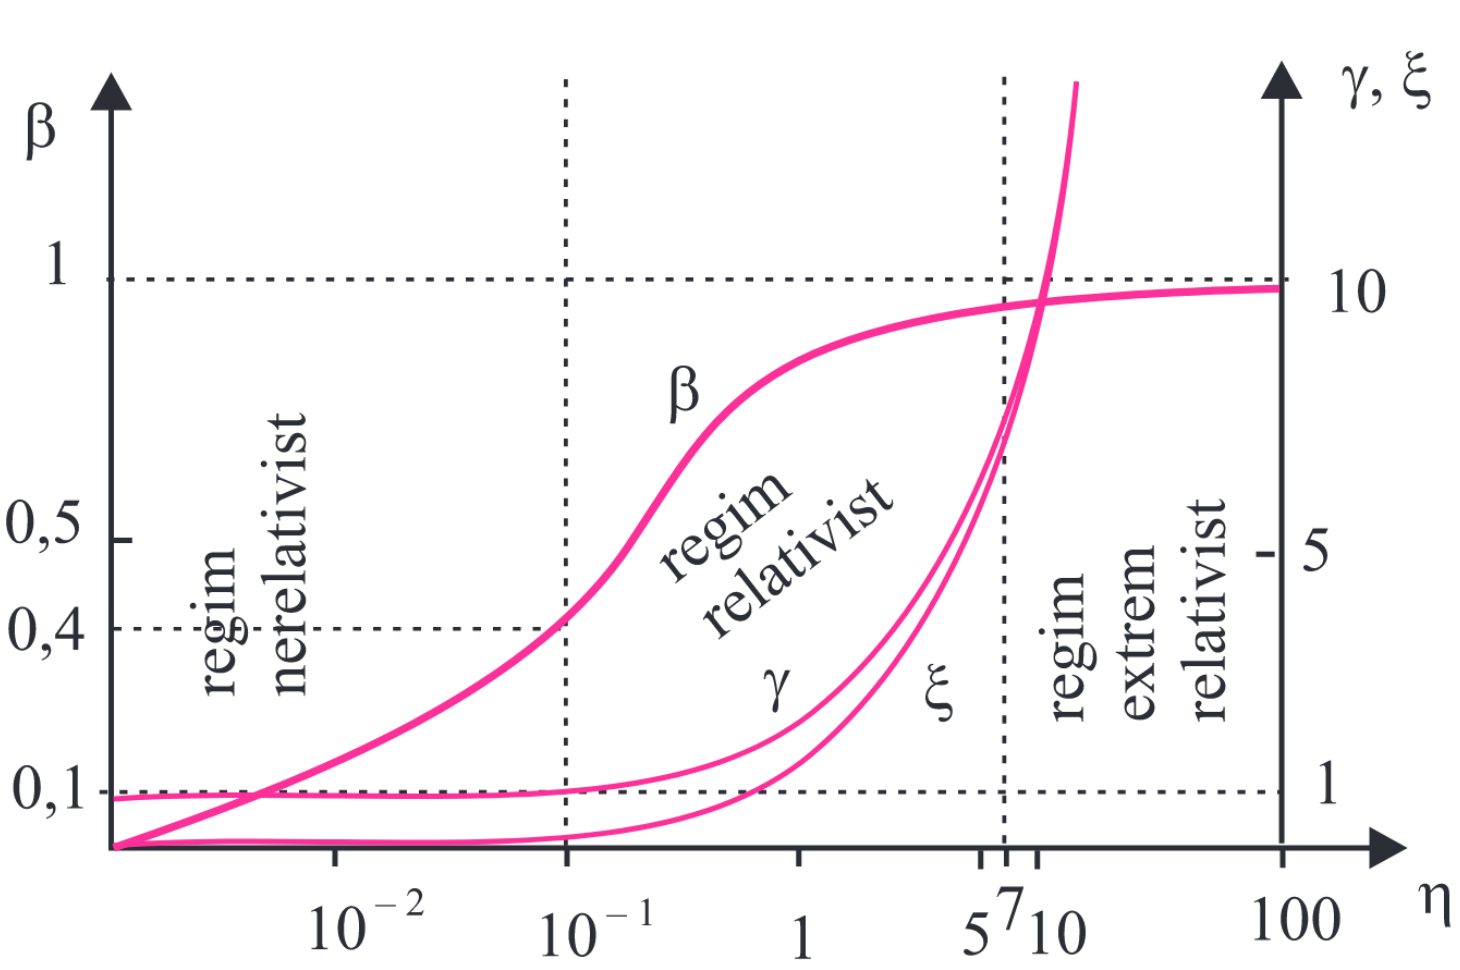
\includegraphics[width=0.45\textwidth]{fig/regimuri}
        \caption{%
            Reprezentare semilogaritmică a dependenței vitezei, energiei, și
            impulsului normate de energia cinetică normată
        }
    \end{wrapfigure}

    În figura 4 este ilustrată variația mărimilor normate $\beta$, $\gamma$,
    și $\xi$ în funcție de energia cinetică normată $\eta$.

    După intervalul cinetic în care iau valori \emph{parametrii reduși}, putem
    delimita trei domenii dinamice:
    \begin{itemize}
        \item domeniul nerelativist, în care masa particulei poate fi considerată
            aproximativ constantă și egală cu masa de repaus
            ($\gamma \approx 1$, $\beta \approx 0,4$).
        \item domeniul relativist, pentru \( 10^{-1} < \eta < 7 \).
        \item domeniul extrem relativist, în care viteza particulei poate fi
            considerată constantă și egală cu viteza luminii ($\beta \approx 1$).
    \end{itemize}
}

În tehnica accelerării particulelor, în fizica atomică și nucleară, se folosesc,
pentru măsurarea energiei și impulsului, unități care nu fac parte din SI, dar
care prezintă avantaje în calculele curente.

Pentru măsurarea energiei unei particule se utilizează de regulă electron-voltul
[eV]. Acesta reprezintă energia câștigată de un electron accelerat sub o
diferență de potențial de 1 V.
\[ 1 ~ \mathrm{eV} = 1,602\cdot10^{-19} ~ \mathrm{J} \]

Deoarece în domeniul extrem relativist impulsul este \( p \approx mc = \frac{E}{c} \),
putem introduce o unitate arbitrară pentru impuls $\left[\frac{eV}{c}\right]$.
\[ 1 \frac{eV}{c} = 5,35\cdot10^{-28} ~ \mathrm{N \cdot s} \]
